\chapter{The key concepts}

\section{Introduction -- random fields, a gentle introduction}

A spatial random field is a \textit{random variable}\index{random variable} that represents spatially continuous phenomena in 2 dimensions. Since this is a difficult concept to grasp this chapter slowly builds up on random variables that are more familiar.


\subsection{A random variable with independent replicates}

You might have come across random variables in other contexts. They are values that are assumed to follow a distribution. 

Random fields do not assume between measurements; the explicitly assume  dependence and include 

\subsection{A random field in 1D}
For the moment assume that we are considering a phenomenon in 1 dimension, for example through time. This could for instance be the temperate in my office. This temperature can easily be measured and since it is cheap to measure the temperature we probably relatively easily set up a system that measures it frequently, say every second over an extended period.  Other measurements could be more expensive and hence can only be measured much less frequently, say 4 times a day. If one wishes to estimate the temperature at a time in-between measurements it can be interpolated from the given values. Figure \ref{fig:ch2:1D} shows an example of this.


% besseres Beispiel finden
% figure showing continuous values
% values measured
% crosses at times when we would like to interpolate

\begin{figure}
\centering
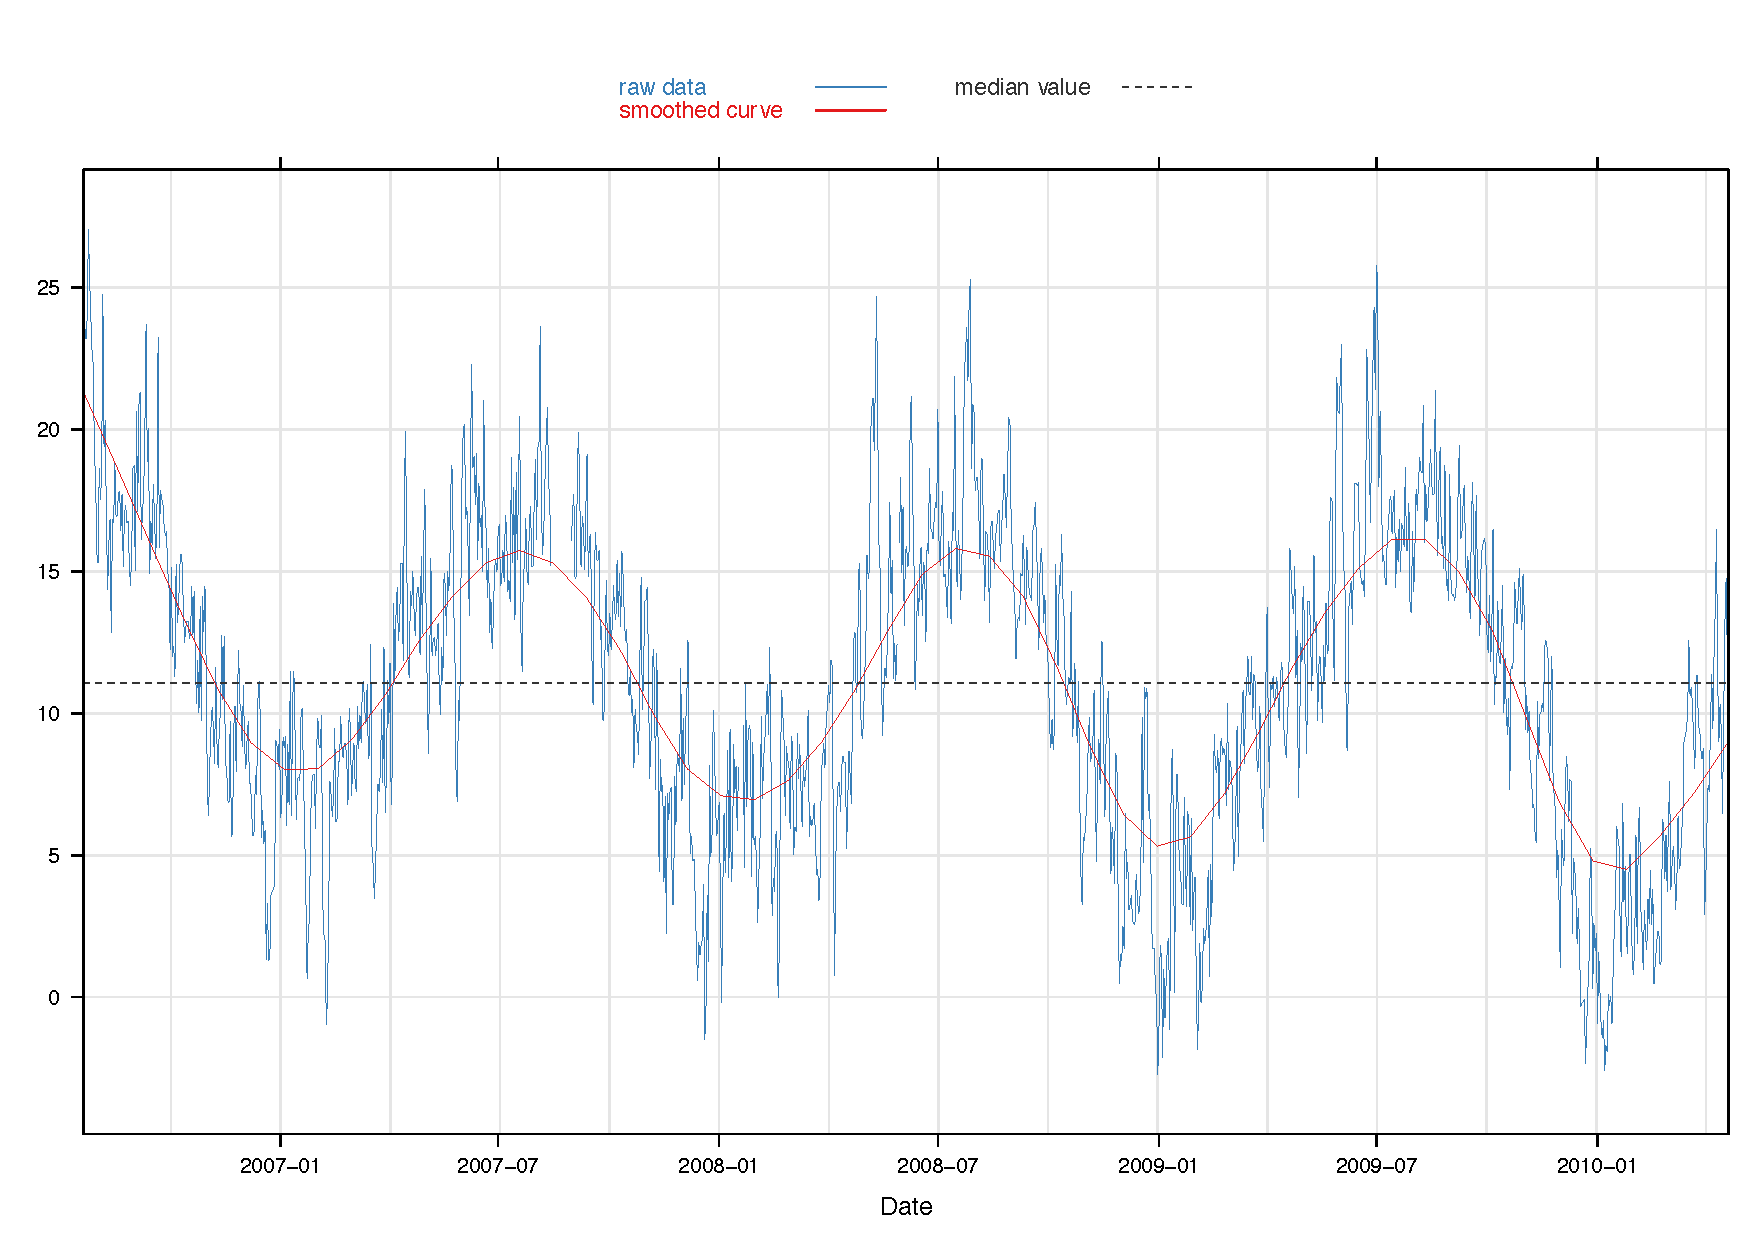
\includegraphics[width=0.3\textwidth]{temp_timeseries}
\caption{\label{fig:ch2:1D} Temperature over time...}
\end{figure}

Clearly, the interpolation should be sensible and be based on the existing measurements. This implies that 
\begin{itemize}
\item realise that observations are not independent through time
\item prediction hence needs to take the other values into account 
\item interpolated values should, on average, be similar to all values measured
\item interpolated values should be similar to values measured close in time
\end{itemize}



random field has properties that describe average behaviour and on distance in time


\subsection{The same thing in 2D}
Lets now move to 2 dimensional space. 

key points:
\begin{itemize}
\item realise that observations are not independent through space
\item interpolated values should, on average, be similar to all values measured
\item interpolated values should be similar values close in space
\end{itemize}

\section{Random fields -- and how they appear everywhere}

Lets have a look at a few examples of data structures.

\subsection{Spatially continuous data as random fields}

\subsection{Spatial point processes, conditional on random fields}

\subsection{Transect data thinned spatial point processes, conditional on random fields}

\section{Random fields -- a definition}

\section{Random fields in practice -- approximating a continuous structure}
\subsection{Approximation by a regular grid}
\subsection{Approximation by a triangulation}

\section{Random fields in practice -- computational challenges}
There are computational challenges with random fields.

\subsection{Why are random fields hard to fit?}

\subsection{INLA}


\section{Spatial point processes}



\section{Thinned point processes}

\subsection{Known thinning process}

\subsection{Unknown thinning process}
\end{document}

% to do:
% find appropriate data set

Consider Figure \ref{fig:elev} which shows the elevation in a rainforest study plot in Panama. In this data structure that  takes on values everywhere in the plot; there is not a single location where it would not make sense to consider elevation as the quantity is spatially continuous.
\begin{figure}
\centering
%\includegraphics[width=0.3\textwidth]{complete}
%\includegraphics[width=0.6\textwidth]{sealsscotland}
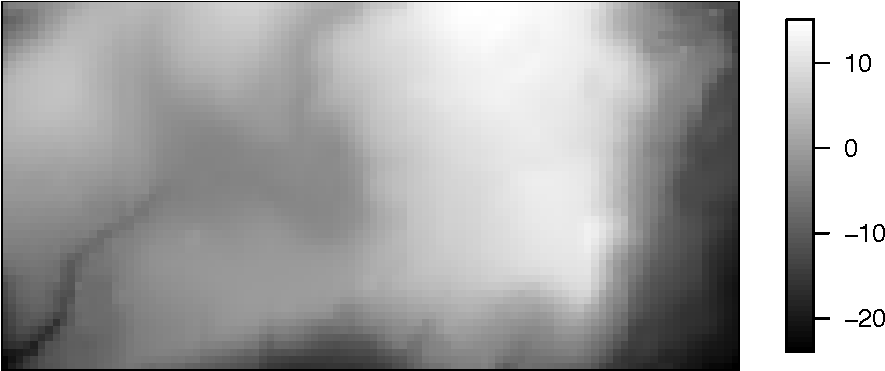
\includegraphics[width=0.6\textwidth]{elev}
\caption{\label{fig:elev} Some elevation somewhere...}
\end{figure}
In practice, however, there are limitations. While there are there are infinitely many locations in even a small area of space the quantity of interest cannot be measured everywhere in space -- and the quantity of interest cannot be fully observed. It can only be measured at a finite number of locations and these location have typically been chosen as part of the study design. There is an interest in interpolating to locations where no measurements have been taken -- referred to as \textit{spatial prediction}. This prediction into other areas of space needs to be done in a clever way, that take into account information from given measurements. In particular, on would like the predicted values to be similar to the values measured in the other locations. The figure is actually based on XX measurements in as many locations randomly distributed across the plot. There might also be an interest in relate one spatially continuous variable to other spatially continuous variables as part of a modelling exercise. These spatial covariates might help to explaining why values are high/low in different areas of the plot, but there might still be spatial structure left that needs to be accounted for.

This data structure is often referred to as \textit{\index{geo-referenced data}} or \textit{\index{geostatistical data}}.

\subsection{Spatial point patterns}
Figure \ref{fig:pattern} which shows  the same rainforest study plot as Figure \ref{fig:elev}, but this time the locations of trees of the species \textit{Beilschmidia} have been plotted. A study might be interested in analysing the pattern formed by those trees to understand habitat preferences of the species. Hence, unlike in the previous example the locations have not been deliberately chosen as part of the study but are the object of interest. The main interest is to understand-- and hence model the spatial pattern.
Again, spatial covariates might explain the spatial pattern but there might still be spatial structure left that needs to be accounted for.

This data structure is referred to as a \textit{\index{spatial point pattern}}.
\begin{figure}
\centering
%\includegraphics[width=0.3\textwidth]{complete}
%\includegraphics[width=0.6\textwidth]{sealsscotland}
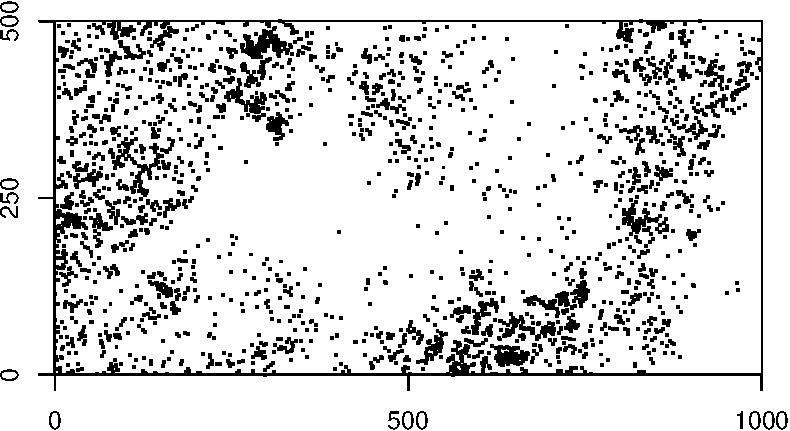
\includegraphics[width=0.6\textwidth]{rain_pattern}
\caption{\label{fig:pattern} Rainforest trees...}
\end{figure}




\subsection{Data collected on transects}
\subsection{Distance sampling data}


\section{Our approach}

How do deal with the random fields in practice


\subsection{Flexible representation of space}

Computationally complex. Hence need to be computationally efficient.

Need to approximate.

Space is complex (sphere, holes) -- need to be flexible. Grids are rigid... 

\subsection{Flexible representation of spatial dependence}

\subsection{Computationally efficient fitting algorithms.}


\section{What to expect from the book}


Finding a rigorous yet flexible way of representing the spatial structure and linking this with computationally efficient model fitting strategies that allow us to fit relevant and realistically complex models.

\section{Structure of the book}

Next Chapter explores key concepts by referring to the different data structures we have seen here. It ends with a roadmap of this book.
 
Chapter after that formalises these concepts

\end{document}



